% Source for docs/static/img/environment-transition.svg. Rebuild from the repository root:
%   pdflatex -output-directory=/tmp docs/scripts/environment-transition.tex
%   pdf2svg /tmp/environment-transition.pdf docs/static/img/environment-transition.svg
%   python3 docs/scripts/prepare_rollout_svgs.py
\documentclass[tikz,border=3pt]{standalone}
\usepackage{amsmath,amssymb,bm}
\usetikzlibrary{arrows.meta,positioning,calc,fit}

\colorlet{agentA}{red!80!black}     % agent 1: policy, prompts, responses, loss
\colorlet{agentB}{blue!80!black}    % agent 2
\colorlet{learned}{orange!80!black} % learned evaluators: critic, reward model
\colorlet{update}{green!50!black}   % gradients and parameter updates

\tikzset{
  >={Stealth[length=3.2pt,width=3pt]},
  box/.style={draw, line width=1pt, inner sep=2.5pt, minimum height=13pt},
  policy/.style={box, rounded corners=3pt, minimum width=30pt},
  flow/.style={->, line width=.8pt},
  note/.style={font=\scriptsize, align=left},
  label/.style={anchor=west, font=\footnotesize},
}

% One environment transition, left to right: the agents' responses at turn t enter the
% external transition, which returns each agent's own observation for turn t+1.
% Columns are animation stages.
\begin{document}
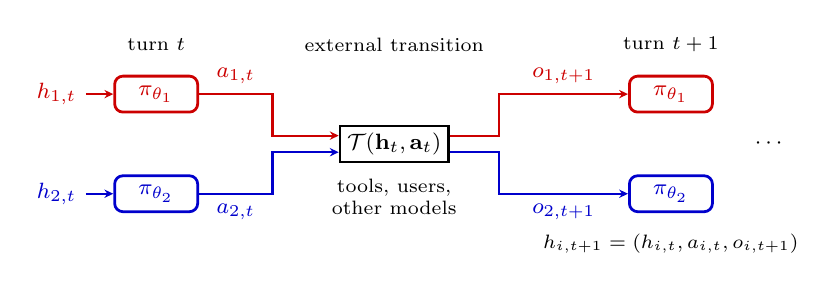
\begin{tikzpicture}[x=1pt, y=1pt, font=\footnotesize]
  % Stage 0: at turn t, each agent's policy acts on its own history.
  \node[note] at (36,36) {turn $t$};
  \node[agentA] (h1) at (0,18) {$h_{1,t}$};
  \node[agentB] (h2) at (0,-18) {$h_{2,t}$};
  \node[policy, agentA] (p1) at (36,18) {$\pi_{\theta_1}$};
  \node[policy, agentB] (p2) at (36,-18) {$\pi_{\theta_2}$};
  \draw[flow, agentA] (h1) -- (p1);
  \draw[flow, agentB] (h2) -- (p2);

  % Stage 1: the responses enter the external transition.
  \node[box] (T) at (122,0) {$\mathcal{T}(\mathbf{h}_t,\mathbf{a}_t)$};
  \node[note] at (122,36) {external transition};
  \node[note, align=center] at (122,-19) {tools, users,\\other models};
  \draw[flow, agentA] (p1.east) -- node[above] {$a_{1,t}$} (78,18) |- ([yshift=3pt]T.west);
  \draw[flow, agentB] (p2.east) -- node[below] {$a_{2,t}$} (78,-18) |- ([yshift=-3pt]T.west);

  % Stage 2: each agent receives its own observation at turn t+1.
  \node[note] at (222,36) {turn $t+1$};
  \node[policy, agentA] (q1) at (222,18) {$\pi_{\theta_1}$};
  \node[policy, agentB] (q2) at (222,-18) {$\pi_{\theta_2}$};
  \draw[flow, agentA] ([yshift=3pt]T.east) -- (160,3) |- node[pos=.75, above] {$o_{1,t+1}$} (q1.west);
  \draw[flow, agentB] ([yshift=-3pt]T.east) -- (160,-3) |- node[pos=.75, below] {$o_{2,t+1}$} (q2.west);
  \node at (258,0) {$\cdots$};
  \node[note] at (222,-36) {$h_{i,t+1}=(h_{i,t},a_{i,t},o_{i,t+1})$};
\end{tikzpicture}
\end{document}
